\chapter{ACL}

\section{ACL Operation Overview}

An ACL contains a sequential list of permit or deny statements, known as access control entrie (ACEs). ACEs are also commonly called ACL statements. 

\subsection{ACEs Logic Operations}

ACLs are processed in a top down manner. When an ACL is inspected, if the information in a packet header and an ACL statement match, the remaining statements are not examined, and the packet is either denied or permitted through as specified by the ACL. \\

If a packet header does not match an ACL statement, the packet is tested against the next statement in the list. This matching process continues until the end of the list is reached. If no conditions match, the address is rejected. In a nut shell, ACL always stops testing conditions after the first match, therefore, the order of the ACEs is critical. \\

At the end of every ACL is a statement is an implicit deny any statement and because of this statement, an ACL should have at least one permit statement in it; otherwise, the ACL blocks all traffic.

\subsection{Inbound and Outbound ACL Logic}

The Figure \ref{InOut} shows the logic of routing and ACL processes. When a packet arrives at a router interface, the router checks for an ACL on the inbound interface. If an ACL exists, the packet is tested against the statements in the list. \\

\begin{figure}[hbtp]
\caption{Inbound and Outbound ACLs}\label{InOut}
\centering
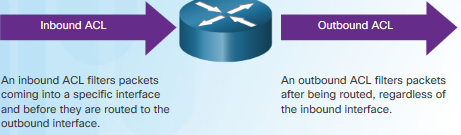
\includegraphics[scale=1]{pictures/InOut.PNG}
\end{figure}

If the packet matches a statement, the packet is either permitted or denied. If the packet is accepted, it is then checked against routing table entries to determine the destination interface. If a routing table entry exists for the destination, the packet is then switched to the outgoing interface, otherwise the packet is dropped. \\

Next, the router checks whether the outgoing interface has an ACL. If an ACL exists, the packet is tested against the statements in the list. If the packet matches a statement, it is either permitted or denied. \\

If there is no ACL or the packet is permitted, the packet is encapsulated in the new Layer 2 protocol and forwarded out the interface to the next device.

\subsection{Numbered and Named ACLs}

Standard and extended ACLs can be created using either a number or a name to identify the ACL and its list of statements.

\paragraph{Numbered ACL} Assign a number based on the following rules:
\begin{itemize}
\item (1 to 99) and (1300 to 1999): Standard ACL
\item (100 to 199) and (2000 to 2699): Extended ACL
\end{itemize}

\paragraph{Named ACL} Assign a name based on the following rules:
\begin{itemize}
\item Cannot contain spaces or punctuation
\item Names are case-sensitive
\item Can contain alphanumeric characters
\item It is suggested that the name be written in CAPITAL LETTER
\end{itemize}

\subsection{ACL configuration guidelines}

\begin{itemize}
\item Create an ACL in global configuration mode and then apply it to interfaces
\item Ensure that the last statement is \code{deny any} or \code{deny ip any any}
\item The statement order is important because ACLs are processed drop-down. As soon as a statement is matched, ACL stops.
\item The most specific ACEs are at the top of the list.
\item New statements are added to an existing ACL.
\item Place \textbf{Standard} ACLs as close to the \textbf{destination} as possible.
\item Place \textbf{Extended} ACLs as close to the \textbf{source} as possible.
\end{itemize}
	
\section{Standard ACL}

\subsection{Overview}

A standard IPv4 ACL can filter traffic based on source IP addresses only. Unlike an extended ACL, it cannot filter traffic based on Layer 4 ports.\\
 
Because standard ACLs do not specify destination addresses, place them as close to the destination as possible. If a standard ACL was placed at the source of the traffic, the \textit{permit} or \textit{deny} will occur based on the given source address no matter where the traffic is destined. 

\subsection{Placement}

In the figure \ref{standardACLex}, the administrator wants to prevent traffic originating in the 192.168.10.0/24 network from reaching the 192.168.30.0/24 network.\\

\begin{figure}[hbtp]
\caption{Standard ACL placement}\label{standardACLex}
\centering
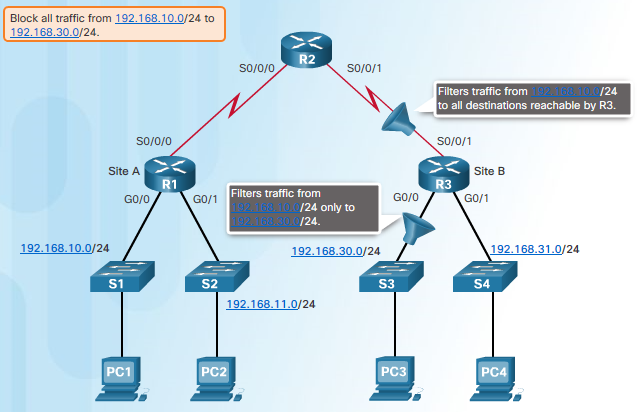
\includegraphics[ width=0.8\textwidth ]{pictures/standardACLex.PNG}
\end{figure}

Following the basic placement guidelines of placing the standard ACL close to the destination, the figure shows two possible interfaces on R3 to apply the standard ACL:

\begin{itemize}
\item R3 S0/0/1 interface - Applying a standard ACL to prevent traffic from 192.168.10.0/24 from entering the S0/0/1 interface will prevent this traffic from reaching 192.168.30.0/24 as well as 192.168.31.0/24 network. Because the intent of the ACL is to filter traffic destined only for 192.168.30.0/24, a standard ACL should not be applied to this interface.

\item R3 G0/0 interface - Applying the standard ACL to traffic exiting the G0/0 interface will filter packets from 192.168.10.0/24 to 192.168.30.0/24. This will not affect other networks that are reachable by R3. Packets from 192.168.10.0/24 will still be able to reach 192.168.31.0/24.
\end{itemize}

\subsection{Examples}

\begin{example}
The following ACL permits a single network. Only traffic from the 192.168.10.0/24 network will be permitted out the Serial 0/0/0 interface.
\begin{verbatim}
access-list 1 permit 192.168.10.0 0.0.0.255
interface s0/0/0
ip access-group 1 out
\end{verbatim}
\end{example}



\section{Extended ACLs}

\subsection{Overview}

Extended ACLs filter packets based on both Source and destination IP addresses, as well as Source and destination TCP and UDP ports. We usually locate extended ACLs as close as possible to the source of the traffic. This way, undesirable traffic is denied close to the source network without crossing the network infrastructure.\\

For example, in figure \ref{extendedACLex}, the administrator wants to deny Telnet and FTP traffic from the .11 network to Company B's 192.168.30.0/24 (.30, in this example) network. At the same time, all other traffic from the .11 network must be permitted to leave Company A without restriction.\\

\begin{figure}[hbtp]
\caption{Extended ACL Placement}\label{extendedACLex}
\centering
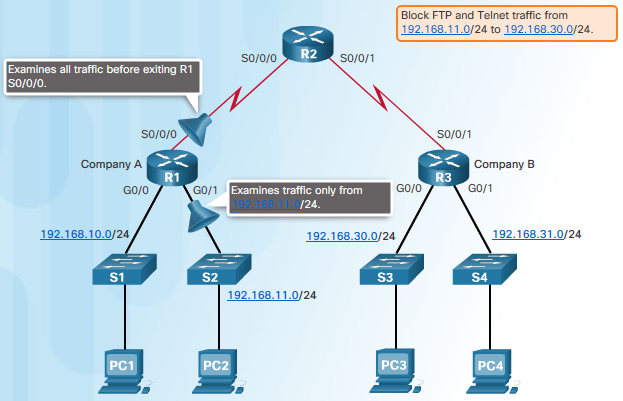
\includegraphics[ width=0.8\textwidth ]{pictures/extendedACLex.PNG}
\end{figure}

A better solution is to place an extended ACL on R1. There are two possible interfaces on R1 to apply the extended ACL:

\begin{itemize}
\item R1 S0/0/0 interface (outbound) - One possibility is to apply an extended ACL outbound on the S0/0/0 interface. Because the extended ACL can examine both source and destination addresses, only FTP and Telnet packets from 192.168.11.0/24 will be denied. Other traffic from 192.168.11.0/24 and other networks will be forwarded by R1. The disadvantage of placing the extended ACL on this interface is that all traffic exiting S0/0/0 must be processed by the ACL including packets from 192.168.10.0/24.

\item R1 G0/1 interface (inbound) - Applying an extended ACL to traffic entering the G0/1 interface means that only packets from the 192.168.11.0/24 network are subject to ACL processing on R1. Because the filter is to be limited to only those packets leaving the 192.168.11.0/24 network, applying the extended ACL to G0/1 is the best solution.
\end{itemize}

\subsection{Established ACL}

With basic standard and static extended access lists, you can approximate session filtering by using the established keyword with the permit command. The established keyword filters TCP packets based on whether the ACK or RST bits are set. (Set ACK or RST bits indicate that the packet is not the first in the session, and therefore, that the packet belongs to an established session.) This filter criterion would be part of an access list applied permanently to an interface.

\subsection{Reflexive ACL}

Unlike Established ACL, which is only used for TCP connection, Reflexive ACLs performs IP session filtering for any type of traffic (TCP, UDP, ICMP, etc.). Reflexive ACLs work by using temporary ACEs inserted into an extended ACL, which is applied on the external interface of the perimeter router. When the session ends or the temporary entry times out, these ACEs are removed from the extended ACL configuration of the external interface. This reduces network exposure to DoS attacks.

\subsubsection{Choosing an Interface: Internal or External} 
Reflexive access lists are most commonly used with one of two basic network topologies. \\

In the first topology (figure \ref{ReflexiveACLex}), reflexive access lists are configured for the external interface Serial 1. This prevents IP traffic from entering the router and the internal network, unless the traffic is part of a session already established from within the internal network.\\

\begin{figure}[hbtp]
\caption{Reflexive Access Lists Configured at the External Interface}\label{ReflexiveACLex}
\centering
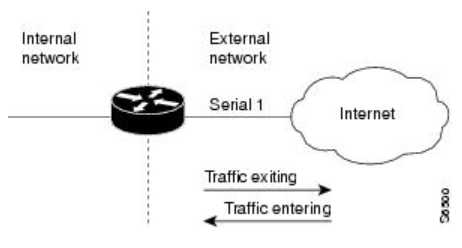
\includegraphics[scale=0.5]{pictures/ReflexiveACLex.PNG}
\end{figure}

In the second topology (figure \ref{ReflexiveACLin}), reflexive access lists are configured for the internal interface Ethernet 0. This allows external traffic to access the services in the Demilitarized Zone (DMZ), such as DNS services, but prevents IP traffic from entering your internal network, unless the traffic is part of a session already established from within the internal network.

\begin{figure}[hbtp]
\caption{Reflexive Access Lists Configured at the Internal Interface}\label{ReflexiveACLin}
\centering
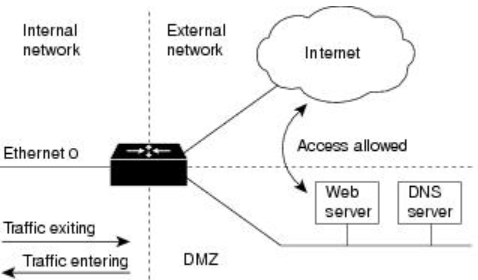
\includegraphics[scale=0.5]{pictures/ReflexiveACLin.PNG}
\end{figure}

\subsubsection{Configuration}

In the previous section, you decided whether to configure reflexive access lists for an internal or external interface. If you choose to configure reflexive access lists for an external interface, perform the following tasks:

\begin{sexylisting}{Reflexive ACL Configured at the External Interface}
ip access-list extended internal-ACL
	permit tcp any any eq 23 reflect telnet-only-reflexive-ACL
	permit udp any any eq 53 reflect dns-only-reflexive-ACL timeout 10
	exit
ip access-list extended external-ACL
	evaluate telnet-only-reflexive-ACL
	evaluate dns-only-reflexive-ACL
	deny ip any any
	exit
interface s0/0/0
	ip access-group internal-ACL out
	ip access-group external-ACL in
	exit
\end{sexylisting}

The internal-ACL only allows Telnet and DNS traffic to exit the network. The external-ACL basically denies all traffic (\code{deny ip any any}). However, whenever a Telnet or DNS traffic is initiated in the internal network, internal-ACL will inform external-ACL about that traffic (\code{reflect}). Receiving information from internal-ACL, external-ACL will add an ACE to allow the return Telnet or DNS traffic (\code{evaluate}).

\subsection{Dynamic ACL (Lock-and-Key Security)}

The benefits and operation of Dynamic ACL are thoroughly explained in the following \href{https://www.youtube.com/watch?v=1EwutKdb6P8&index=2&list=PLyykP25PsLMKk1cKoCtEzRTsjuJ0rbbhl }{links}. The following process summarizes Dynamic ACL operation:

\begin{enumerate}
\item A remote user want to user resources located in the internal network. He/She must open a Telnet or SSH connection to the router to authenticate.
\item The router receives the Telnet/SSH packet, opens a Telnet/SSH session, prompts for a password, and performs a user authentication process. 
\item If the authentication is successful, the Telnet or SSH connection is terminated, and the router creates a
temporary ACE in the dynamic ACL, which provides the user with limited access to the internal resources.
\item The user can now access the internal resources that would otherwise be denied without the dynamic ACL entry.
\item The router deletes the temporary ACE when a configured timeout is reached, or when the system administrator manually clears it. The configured timeout can either be an idle timeout or an absolute timeout. 
\end{enumerate}

\begin{sexylisting}{Dynamic ACL (local database)}
username student secret cisco

access-list 101 permit tcp any host 10.2.2.2 eq telnet
access-list 101 dynamic MyACL timeout 15 permit ip 192.168.10.0 0.0.0.255 192.168.30.0 0.0.0.255
int s0/0/0
	ip access-group 101 in
	exit
	
line vty 0 4
	login local
	autocommand access-enable host timeout 5
	exit
\end{sexylisting}

The \code{autocommand} command configures the system to automatically execute a specified privileged EXEC command when a user connects to a particular line. \\

To test this out, let's try to ping 192.168.30.0/24 network from any host in 192.168.10.0. The output of the ping would be \texttt{Destination host unreachable}. If you want to get access to 192.168.30.0/24 network, you have to authenticate yourself by opening the command prompt and type \texttt{telnet 10.2.2.2}. After typing correct username and password, you can now ping the 192.168.30.0/24 network as normal. However, after 15 minutes (\code{timeout 15}) no access is allowed anymore.\\

\subsection{Examples}

\begin{example}
The following named access list HQServer prevents any computers attached to the g0/0 interface of the Branch router from accessing HQServer (172.16.0.1). All other traffic is permitted.
\begin{verbatim}
ip access-list extended HQServer
  deny ip any host 172.16.0.1
  permit ip any any
  exit
int g0/0
  ip access-group HQServer in
\end{verbatim}
\end{example}

\begin{example}
The following access list BranchServer prevents any computers attached to the g0/0 interface of the HQ router from accessing the HTTP and HTTPS service of the Branch server (172.16.128.1/20). All other traffic is permitted.
\begin{verbatim}
ip access-list extended BranchServer
  deny tcp any host 172.16.128.1 eq 80
  deny tcp any host 172.16.128.1 eq 443
  permit ip any any
  exit
int g0/0
 ip access-group HQServer in
\end{verbatim}
\end{example}

\begin{example}
The access list 103 allows users from the  internal network (192.168.10.0/24) to send both HTTP and HTTPS. The access list 104 allows any TCP traffic from the Internet that was initiated from the hosts in the internal networks to pass (with the \code{established} keyword). These access lists will restrict 192.168.10.0 to allow only website browsing.
\begin{verbatim}
access-list 103 permit tcp 192.168.10.0 0.0.0.255 any eq 80
access-list 103 permit tcp 192.168.10.0 0.0.0.255 any eq 443
access-list 104 permit tcp any 192.168.10.0 0.0.0.255 established
int s0/0/0
	ip access-group 103 out
	ip access-group 104 in
\end{verbatim}
\end{example}

\begin{example}
Configure an extended IPv4 ACL named INTOHQ such that: 
\begin{itemize}
\item Allow any hosts from the Internet to access the County DNS Svr. There should be two ACEs, one for TCP and the other UDP. Both use port 53.
\item Allow any hosts from the Internet to access the County Web Svr. Only port 80 is needed.
\item Allow return TCP traffic from the Internet that was initiated from the hosts in the Central networks to pass (with the established keyword).
\item Apply the ACL to the Central S0/0/0 interface.
\end{itemize}
\begin{verbatim}
ip access-list extended INTOHQ
  permit tcp any host 172.16.10.5 eq 53
  permit udp any host 172.16.10.5 eq 53
  permit tcp any host 172.16.10.10 eq 80
  permit tcp any any established
  exit
int s0/0/0
  ip access-group INTOHQ in
\end{verbatim}
\end{example}

\begin{example}
Configure an extended ACL named SNMPACCESS such that 
\begin{itemize}
\item The SNMP operation runs UDP on port 161.
\item Allow only the County-Admin-PC to access the Central router for the SNMP connection.
\item SNMP connections from other hosts on the Central LAN should fail.
\item Allow all other IP traffic.
\item Apply this ACL on the Central router, G0/0 interface.
\end{itemize}
\begin{verbatim}
ip access-list extended SNMPACCESS
  permit udp host 192.168.10.5 host 192.168.10.1 eq 161
  deny udp any host 192.168.10.1 eq 161
  permit ip any any
  exit
 interface g0/0
  ip access-group SNMPACCESS in
\end{verbatim}
\end{example}

\subsection{Mitigate attacks}

ACLs can be used to mitigate IP address spoofing and denial of service (DoS) attacks (figure \ref{AntispoofingACL}). Use ACL to block inbound packets from the following addresses:

\begin{itemize}
\item All zeros addresses
\item Broadcast addresses
\item Local host addresses (127.0.0.0/8)
\item Reserved private addresses (prevent the spoofing of internal networks)
\item IP multicast address range (224.0.0.0/4)
\end{itemize}

\begin{figure}[hbtp]
  \caption{Antispoofing with ACLs}\label{AntispoofingACL}
  \centering
  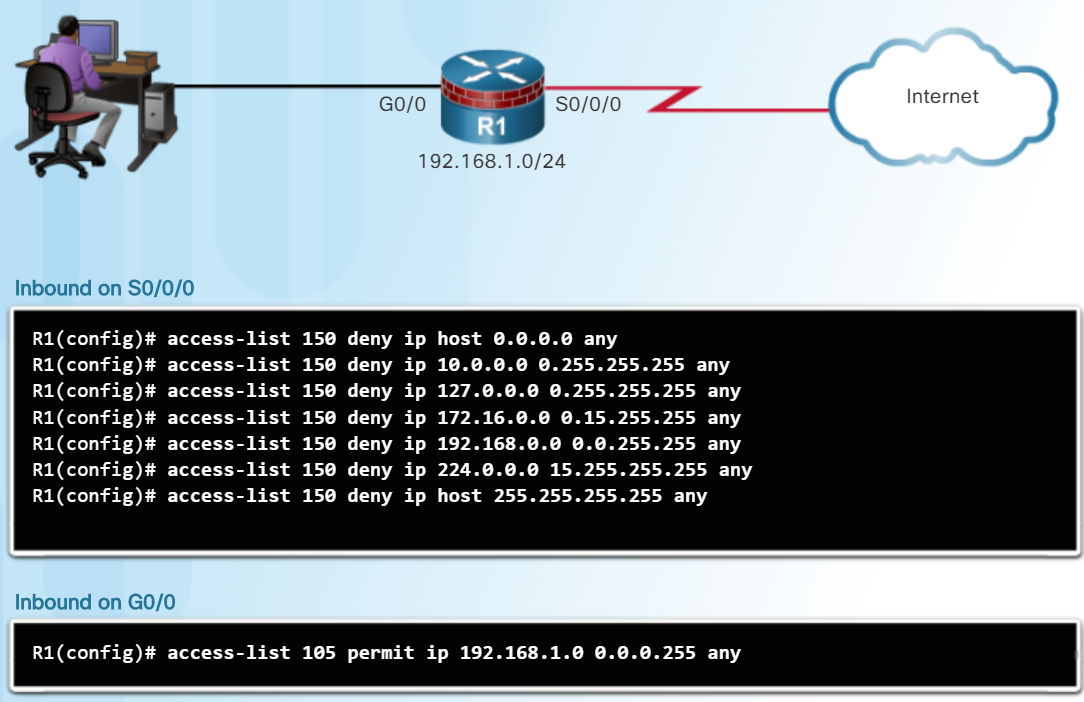
\includegraphics[width=10\xm]{pictures/AntispoofingACL.PNG}
  \end{figure}

Hackers can use ICMP echo packets (pings) to discover network, generate DoS flood attacks, or alter host routing tables. Both ICMP echo and redirect messages should be blocked \emph{inbound} by the router. Several ICMP messages are recommended for proper network operation and should be allowed into the internal network:

\begin{itemize}
\item Echo reply -- Allows users to ping external hosts.
\item Source quench -- Requests that the sender decrease the traffic rate of messages.
\item Unreachable -- Generated for packets that are administratively denied by an ACL.
\end{itemize}

Several ICMP messages are required for proper network operation and should be allowed to exit the network (outbound ACL):

\begin{itemize}
\item Echo -- Allows users to ping external hosts.
\item Parameter problem -- Informs the host of packet header problems.
\item Packet too big -- Enables packet maximum transmission unit (MTU) discovery.
\item Source quench -- Throttles down traffic when necessary.
\end{itemize}

\note Traffic that originates within a router such as pings from a command prompt, remote access from a router to another device, or routing updates are not affected by outbound access lists. The traffic must flow through the router in order for the router to apply the ACEs.

\section{IPv6 ACLs}

In IPv4 there are two types of ACLs, standard and extended and both types of ACLs can be either numbered or named ACLs. With IPv6, there is only one type of ACL, which is equivalent to an IPv4 extended named ACL. An IPv4 ACL and an IPv6 ACL cannot share the same name. There are three significant differences between IPv4 and IPv6 ACLs:

\begin{itemize}
\item The command used to apply an IPv6 ACL to an interface is \texttt{ipv6 traffic-filter} command.
\item IPv6 ACLs do not use wildcard masks but instead specifies the prefix-length
\item Besides \texttt{deny ipv6 any any}, An IPv6 ACL adds two implicit permit statements at the end of each IPv6 access list: \texttt{permit icmp any any nd-na} and \texttt{permit icmp any any nd-ns}
\end{itemize}
	
Because IPv6 ACLs must be configured with both a source and a destination, they should be applied closest to the source of the traffic.

\begin{example}
The access list NO-B1 prevents any IPv6 traffic originating on B1 (2001:DB8:ACAD:B1::2/64) to reach the BranchServer (2001:DB8:ACAD:B2::3/64).
\begin{verbatim}
ipv6 access-list NO-B1
  deny ipv6 host 2001:DB8:ACAD:B1::2 host 2001:DB8:ACAD:B2::3
  permit ipv6 any any
  exit
int g0/1
  ipv6 traffic-filter NO-B1 out
\end{verbatim}
\end{example}



\section{Troubleshoot}

Using the \texttt{show access-lists} command to reveal most of the common ACL errors. The most common errors are entering ACEs in the wrong order and not applying adequate criteria to the ACL rules. Following these steps to troubleshoot ACL:

\begin{enumerate}
\item Check the criteria of ACL rules
\item Check the order of ACEs
\item Check the direction of ACL (inbound, outbound)
\item Check the location of ACL (which router, which interface). Remember that extended ACLs are placed as close as possible to the source and standard ACLs are placed as close as possible to the destination.
\end{enumerate}

\begin{example}
The 192.168.10.0/24 network cannot use TFTP to connect to the 192.168.30.0/24 network.
\begin{verbatim}
R3# show access-lists 120
Extended IP access list 120
    10 deny tcp 192.168.10.0 0.0.0.255 any eq telnet
    20 deny tcp 192.168.10.0 0.0.0.255 host 192.168.31.12 eq smtp
    30 permit tcp any any
\end{verbatim}
Statement 30 in access list 120 allows all other TCP traffic. However, because TFTP uses UDP instead of TCP, it is implicitly denied. Recall that the implied \code{deny any} statement does not appear in show access-lists output and therefore matches are not shown. Statement 30 should be \code{permit ip any any}.
\end{example}


\begin{example}
The 192.168.11.0/24 network can use Telnet to connect to 192.168.30.0/24, but this connection should not be allowed. The results of the \code{show access-lists 130} command indicate that the permit statement has been matched.
\begin{verbatim}
R1# show access-lists 130
Extended IP access list 130
    10 deny tcp any eq telnet any
    20 deny tcp 192.168.11.0 0.0.0.255 host 192.168.31.12 eq smtp
    30 permit tcp any any (12 match(es))
\end{verbatim}
The 192.168.11.0/24 network can use Telnet to connect to the 192.168.30.0/24 network because statement 10 currently denies any source packet with a port number that is equal to Telnet. To deny Telnet traffic inbound on G0/1, deny the destination port number that is equal to Telnet. The statement 10 should be \code{deny tcp 192.168.11.0 0.0.0.255 192.168.30.0 0.0.0.255 eq telnet}.
\end{example}